\subsection{Interfejs}
W pierwszej iteracji, na podstawie przedstawionych przez zamawiającego założeń, przygotowałem wstępny projekt interfejsu aplikacji. Poniżej przedstawiam pierwszą wersję aplikacji:

% logowanie v1 
\begin{figure}[H]
\centering
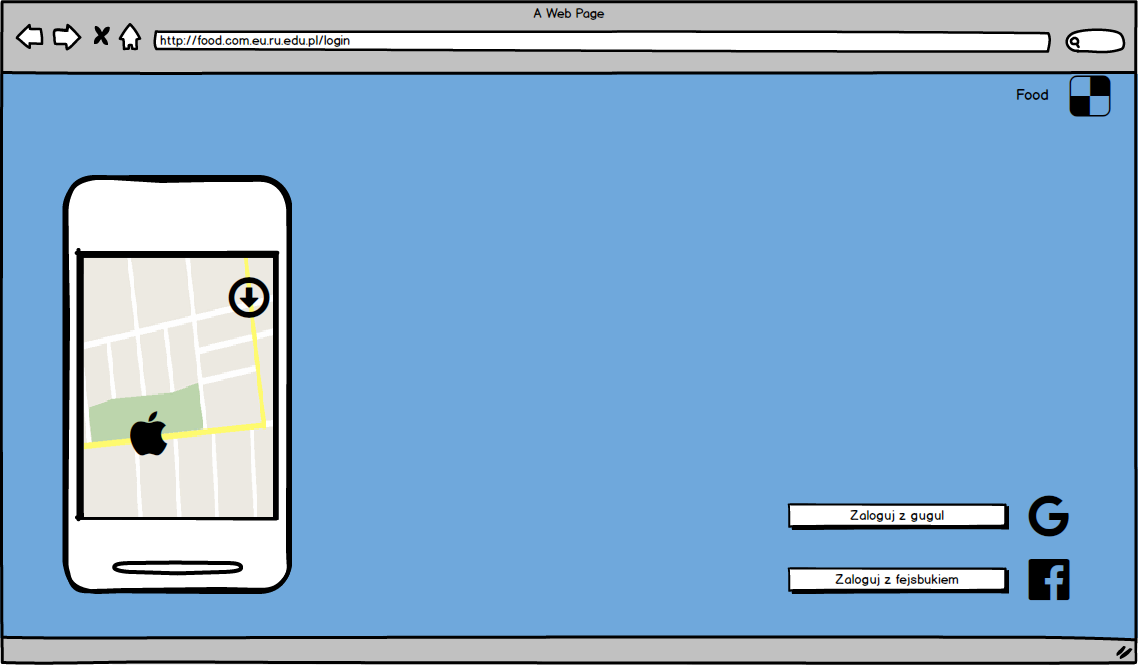
\includegraphics[width=15cm]{pictures/Logowanie_v0.png}
\caption{Ekran logowania}
\end{figure}

% lista produktów v1 
\begin{figure}[H]
\centering
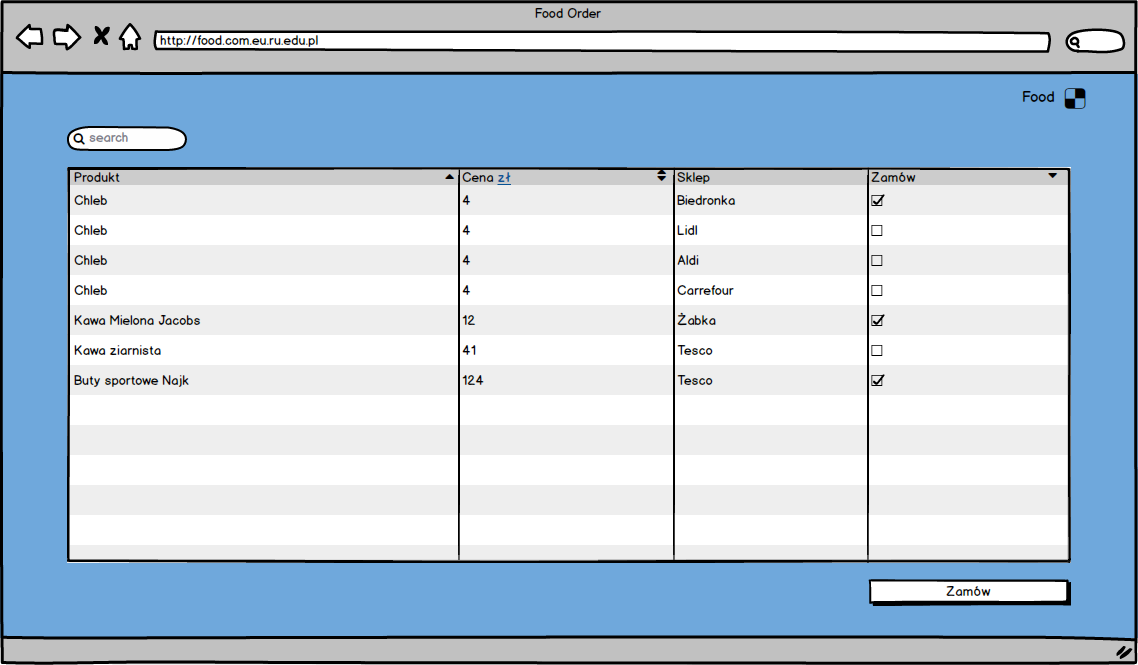
\includegraphics[width=15cm]{pictures/Lista_produktow_v1.png}
\caption{Ekran wyboru listy produktów}
\end{figure}

% lista produktów v1 
\begin{figure}[H]
\centering
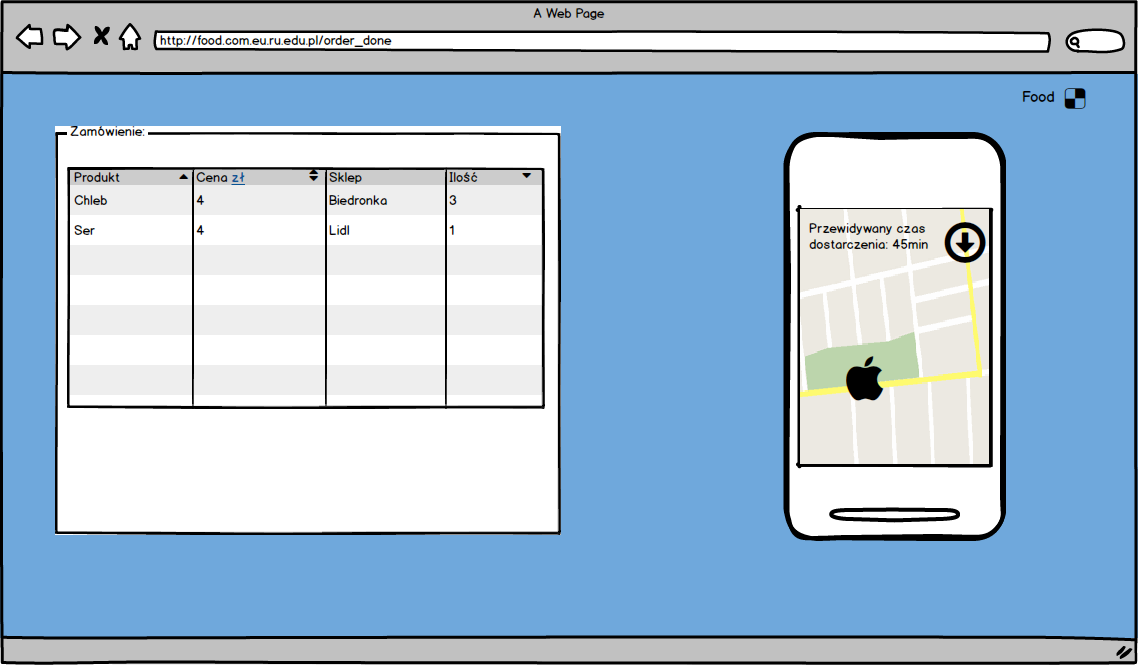
\includegraphics[width=15cm]{pictures/Zamowienie_zlozone_v1.png}
\caption{Ekran przedstawiający informację o złożonym zamówieniu i przewidywanym czasie dostawy}
\end{figure}

\subsection{Uwagi zamawiającego}
Po przedstawieniu zamawiającemu pierwszej wersji interfejsu, stwierdził on, iż aplikacja ma właściwą szatę kolorystyczną. Chciałby jednak, aby lista produktów była wykonana w bardziej przejrzysty i łatwiejszy w obsłudze sposób. W pierwszej iteracji zostały przedstawione zamawiającemu najważniejsze okna w systemie.
